%%%%
%% Copyright 2022 Pierre S. Caboche
%% All rights reserved
%%%%

\part{\TeXstudio} \label{texstudio}


\TeXstudio\ is my editor of choice for editing a \LaTeX\ document, an \emph{``integrated writing environment for creating \LaTeX"} whose goal is to \emph{``make writing \LaTeX\ as easy and comfortable as possible."} \citep{texstudio} \\

 Let's have a quick look at it\dots

\section{The interface}

Here is what the interface of \TeXstudio\ typically looks like when in use:

\begin{figure}[h]
	\caption{The \TeXstudio\ interface}
	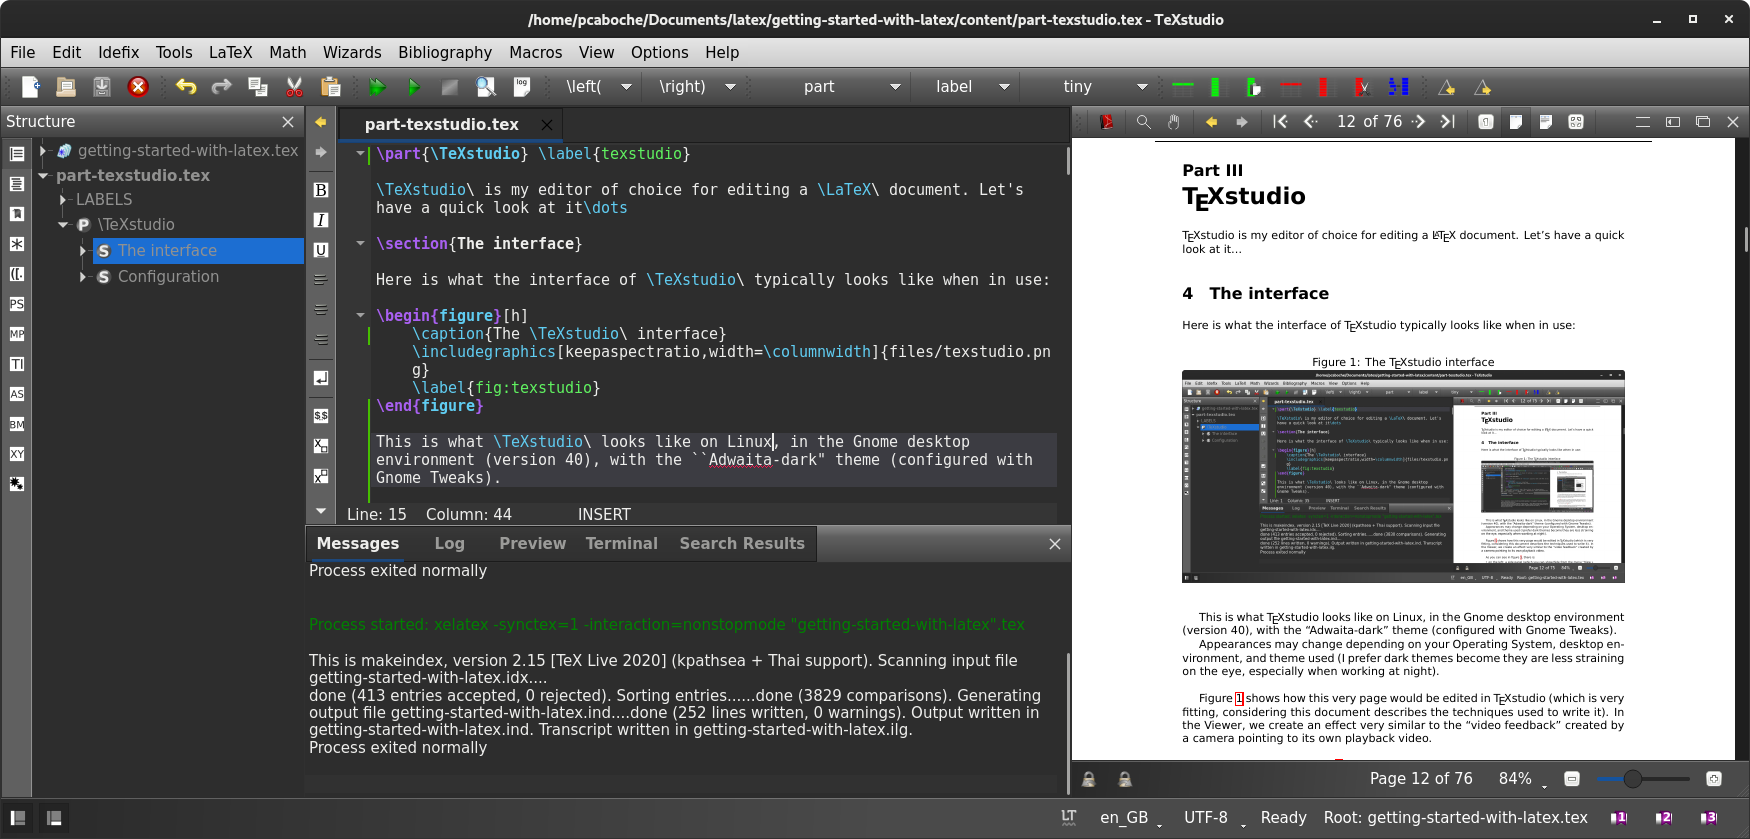
\includegraphics[keepaspectratio,width=\columnwidth]{files/texstudio.png}
	\label{fig:texstudio}
\end{figure}

This is what \TeXstudio\ looks like on Linux, in the Gnome desktop environment (version 41), with the dark theme configured (I find dark themes less straining on the eyes, especially when writing late at night).

Appearances may change depending on your Operating System, desktop environment, and theme used. \\

Figure \ref{fig:texstudio} shows how this very page would be edited in \TeXstudio\ (which is very fitting, considering this document describes the techniques used to write it). In the Viewer, we create an effect very similar to the ``video feedback" created by a camera pointing to its own playback video. \\

As you can see in figure \ref{fig:texstudio}, there is:
\begin{itemize}
	\item on the left: a side panel (which you can show/hide from the menu ``View >> Show >> Side Panel") that will show you the structure of the document, give you access to some \LaTeX\ commands shortcuts, etc.
	\item in the center: the editor for your \LaTeX\ code. \\
	At the bottom of it, you will find a panel for the messages and logs
	\item on the right: the generated document, which will appear after you generate the document from your \LaTeX\ files, by clicking the ``Build \& View" button (or by pressing F5)
	\begin{figure}[h]
		\caption{The ``Build \& View" button (F5)} \label{fig:build-and-view}
		\centering
		
\includegraphics[keepaspectratio,width=2em]{files/build-and-view.png}
	\end{figure} 
\end{itemize}

\TeXstudio\ is best enjoyed on a fairly wide screen (just like many other code editors, where you often have several views side by side). \\

\bigskip

\subsection{Build \& View, Go to Source} \label{build-and-view}

When in the editor, clicking on the ``Build \& View" button (figure \ref{fig:build-and-view}) will generate the document, and highlight the object corresponding to the code where your cursor was in the editor. \\

Similarly, in the editor, select some code, do a right-click, select the ``Go to PDF" option, and \TeXstudio\ will show you the location of the object in the generated document (based on the position of your cursor, not where you performed your right click). \\

Conversely, in the document viewer, do a right-click on any part of the document, select the ``Go to Source" option, and \TeXstudio\ will open the source file, and place the cursor on the code that generated that part of the document (i.e. where you performed the right click). \\

These options make it very easy to navigate between the \LaTeX\ code and the generated document.



\bigskip

\subsection{Toggle Comments}

In \TeXstudio, it is very easy to comment and uncomment parts of the source code.

\begin{itemize}
	\item select the code you want to comment or uncomment
	\item toggle the comments with the ``Ctrl + T" shortcut
\end{itemize}

We will see the importance of comments in the writing process in section ``\longref{comments}". Notably, you can put as many comments as you want in a \LaTeX\ document, so you don't need to discard any draft idea: just comment them out. You'll remove the comment only when you are sure it is not relevant anymore.

\bigskip


\subsection{Undo, Redo}

Like with many editors, ``Undo" in \TeXstudio\ is performed with the ``Ctrl + Z" shortcut. \\
However, please keep in mind that the shortcut for ``Redo" is ``Ctrl + Shift + Z". \\


\bigskip

\subsection{Code completion}

Like with many source code editors, \TeXstudio\ provides some code completion that is tailored specifically for \LaTeX, for example:
\begin{itemize}
	\item commands \\
	Any string starting with \texttt{\textbackslash} will show you a list of possible commands
	
	\item environments \\
	Any string starting with \texttt{\textbackslash begin\{} will show you a list of possible environments
	
	\item references\\
	Typing \texttt{\textbackslash ref\{}, \texttt{\textbackslash nameref\{}, or \texttt{\textbackslash pageref\{} will show a list of available label (see ``\longref{cross-references}")
	
	\item etc.
\end{itemize}



\bigskip

\subsection{Code highlights}

\TeXstudio\ will highlight:
\begin{itemize}
	\item the syntax
	\item words that may be spelled incorrectly (in red squiggly underline)
	\item words that are repeated within a short distance of each other (in yellow squiggly underline)
	\item duplicate labels (in orange)
	\item references that point to non-existing labels (in green squiggly underline)
	\item etc.
\end{itemize}


\subsection{And so much more!}

If you explore the interface of \TeXstudio, you will see that there are many features to fit the needs of different \LaTeX\ users (to the point that it can be really overwhelming at the beginning). \\

I have decided to focus on a few features: the ones that are most universally used, and the ones that are the most useful, especially at the beginning. % (e.g. being able to see the relation between the code and the generated document, as described in section \ref{build-and-view}, really improves productivity!) 
\\

At the core, the interface of \TeXstudio\ is very straightforward: an editor, a document viewer, the ability to jump between the two (as described in section \ref{build-and-view}, a feature that really improves productivity!), code completion, different types of highlights (syntax, references, typos), etc. The workflow (in which we generate a document from \LaTeX\ code) is quite different from other text processors, but we get used to it fairly rapidly. \\

Now that we have a better understanding of what \TeXstudio\ is, and why this is our editor of choice, our next step will be to install all of the necessary software for editing in \LaTeX\dots

\bigskip

\section{Configuration}


\subsection{Configuring \TeX studio}


Go to ``Option >> Configure TeXstudio\dots". A window appears. \\
Select the ``Build" tab


\begin{figure}[h]
	\caption{\TeXstudio's configuration}
	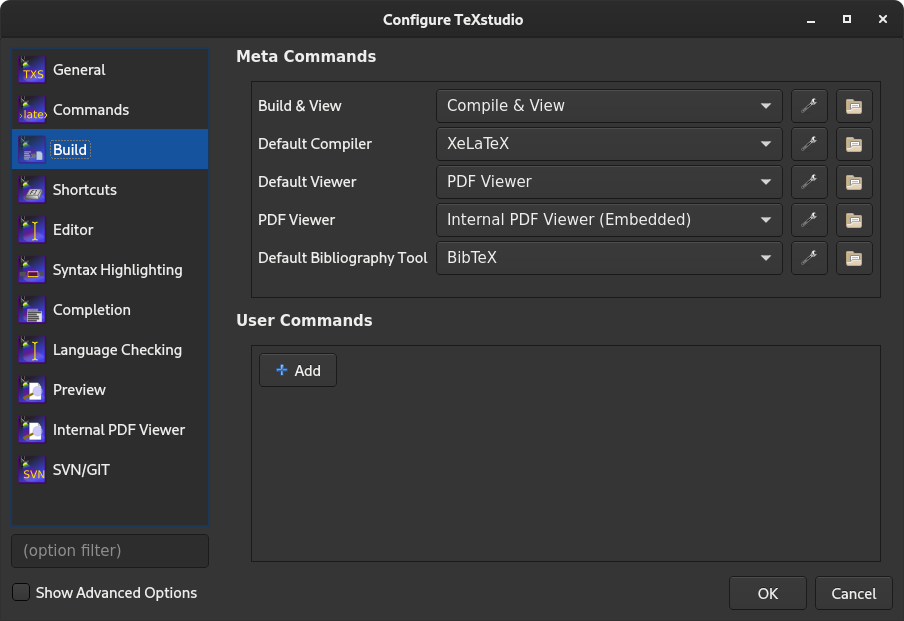
\includegraphics[keepaspectratio,width=\columnwidth]{files/texstudio-configure-embedded.png}
	\label{fig:texstudio-configure-embedded}
\end{figure}


In this screen, we configure the following:

\begin{itemize}
	\item we set ``Default Compiler" to ``XeLaTeX" \\
	This way, we will be able to use the fonts installed on our system
	
	\item we set ``PDF Viewer" to ``Internal PDF Viewer (Embedded)" \\
	This is the default
	
	\item we set ``Default Bibliography Tool" to ``BibTeX" \\
	Needed for section \ref{apa-biblio}
	
\end{itemize}


\subsection{Windowed mode}

There are several reasons why you might prefer to open the PDF Viewer in Windowed mode rather than Embedded mode. For example, your screen might not be wide enough, or you may want to display the PDF Viewer in a secondary screen. \\

Here is how to configure the PDF Viewer in Windowed mode (this setting will apply even after you restart \TeXstudio):

\begin{itemize}
	\item Go to ``Option >> Configure TeXstudio\dots". A window appears. \\ 
	Select the ``Build" tab, then set ``PDF Viewer" to ``Internal PDF Viewer (Windowed)", as shown in figure \ref{fig:texstudio-configure-windowed}
	
	\item If the PDF Viewer is already opened, then close it
	
	\item Press the ``Build \& View" button (figure \ref{fig:build-and-view}), and the ``PDF Viewer" will open in Windowed mode
\end{itemize}




\begin{figure}[h]
	\caption{Setting up \TeXstudio's Viewer in Windowed mode}
	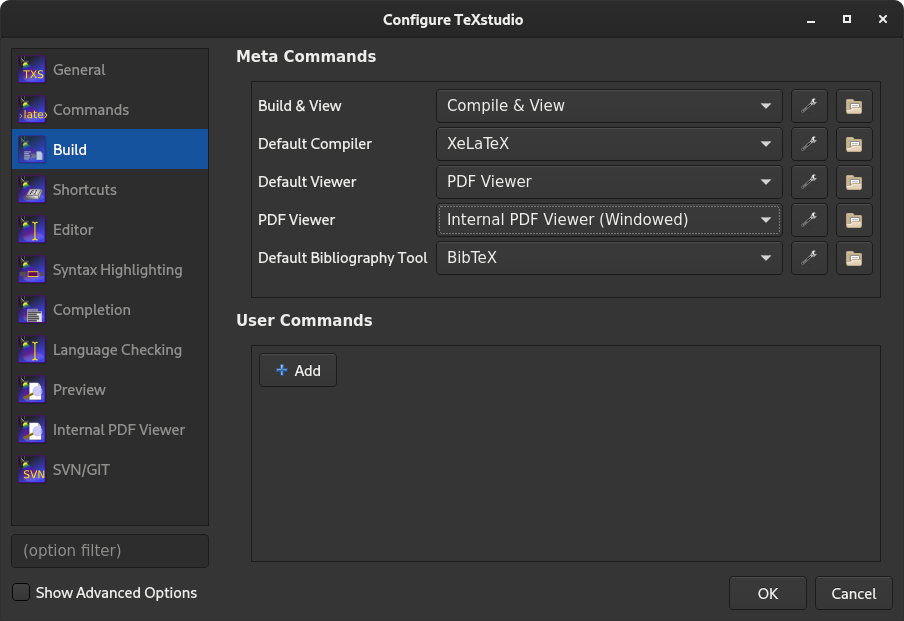
\includegraphics[keepaspectratio,width=\columnwidth]{files/texstudio-configure-windowed.png}
	\label{fig:texstudio-configure-windowed}
\end{figure}


If the PDF Viewer was already in Embedded mode and you want to put it Windowed mode, then press the button highlighted in figure \ref{fig:windowed-viewer} (note that this will not save the setting for after you restart \TeXstudio)

\begin{figure}[h]
	\caption{Windowed Viewer}
	\centering
	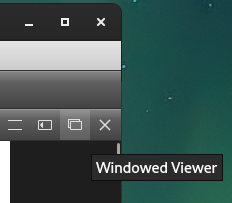
\includegraphics[keepaspectratio,width=6cm]{files/Windowed-Viewer.png}
	\label{fig:windowed-viewer}
\end{figure}


